\documentclass[a4paper,12pt]{article}
\linespread{1.5}
\usepackage[left=2cm,top=2cm,right=2cm,bottom=2cm]{geometry}

%\usepackage{palatino}

\usepackage{xypic}
\usepackage{natbib}
\bibliographystyle{plainnat}
\bibpunct{[}{]}{;}{s}{,}{,}

\usepackage[header,page,titletoc]{appendix}
\renewcommand{\appendixname}{Appendix}
%\renewcommand{\appendixtocname}{List of appendices}

\usepackage[colorlinks=true,linkcolor=black,citecolor=black,filecolor=black,menucolor=black,urlcolor=black]{hyperref}
\usepackage{graphicx}
\usepackage{amsmath}
\usepackage{pdfpages}
\usepackage{wrapfig}
\usepackage{fancyhdr}
\usepackage{pict2e}
\setlength{\headheight}{15.2pt}

\pagestyle{fancy}
\usepackage{cite}
%
% fix citations to be IEEE style
\def\citepunct{], [}
\def\citedash{]--[}

\newcommand{\nonumsection}[1]{
\section{#1}
%\addcontentsline{toc}{section}{#1}
}


\newenvironment{packed_itemize}{
\begin{itemize}
  \setlength{\itemsep}{1pt}
  \setlength{\parskip}{0pt}
  \setlength{\parsep}{0pt}
}{\end{itemize}}

%Used to change "Abstract" to "Executive Summary"

% Paragraph Settings
\setlength{\parindent}{0pt}
\setlength{\parskip}{5pt}

\begin{document}
\thispagestyle{empty}
\vspace*{\fill}

\includegraphics[width=10cm]{./UofAlogo.pdf}\\
\noindent
\textsc{
\textsc{School of Electrical \& Electronic Engineering}\\
Adelaide, South Australia, 5005\\ \\
}
\noindent
\Large{\textbf{
ELEC ENG 4039A/B \\
Honours Project\\
	}}
	\Large{
		A Radio Relay System for Remote Sensors in the Antarctic \\
	}
	\small{\textbf{Supervisors: Dr. Chris Coleman, Dr Said Al-Sarawi}}
	\ \\
	\ \\
	\Large{\textbf{
		Final Report \\
	}}
	\ \\
	\small{\textbf{
		Written by: \\}
		Mark Jessop \\
		1163807
	}
	\ \\
	\ \\
	Date Submitted: October 22, 2010 \\
	Signature of Supervisor: \\
 %\end{center}
 \vspace*{\fill}

\newpage
 \thispagestyle{empty}
 \vspace*{\fill}
\begin{abstract}
\noindent
A common problem with remote sensor systems is the retrieval of data. Satellite-based systems are expensive, as is travelling to the sensor. HF propagation provides an inexpensive alternative. Radio signals below 30MHz can easily bounce off the ionosphere, travelling thousands of kilometres using only a few watts of transmit power.
Based around an Atmel XMega Micro-Controller and using Direct Digital Synthesis techniques, this project aims to provide a reliable low power HF telemetry system, usable in a variety of remote telemetry applications. 
By making use of the XMega's power-save modes and using high-efficiency RF amplifiers, power consumption is minimised, allowing months of operation from battery power.
\end{abstract}
\vspace*{\fill}
\newpage
\tableofcontents
\newpage

\section{Introduction}
Many scientific experiments require data logging over a long time period, and in remote locations. To further research progress, it is desirable for some of the collected data to be accessible throughout the run of the experiment.

A number of solutions exist to obtain data from a remote sensor unit. The first is to physically access the remote sensor station, and copy data from whatever storage may exist. For very remote sensor units visiting the site may be impractical or too costly, so some form of wireless communication is often used. 

Satellite data transmission is a reliable way of retrieving data, but comes at a high cost. For example, using the Iridium Satellite constellation to transmit data would cost approximately USD\$2.50 per minute, with a 2400 baud data rate\citep{ref:iridium}.

The other option is to other methods of radio communication. For reasonably short ($<$50km) distances VHF or UHF telemetry can be used. For example, the Australian Bureau of Meteorology uses a network of VHF transmitters\citep{ref:bomtx} and repeaters to obtain data from weather stations around Adelaide. VHF and UHF can work for longer distances ($>$50km), but with less reliability. Transmission at these distances relies on tropospheric ducting, a phenomenon that is not always present. To obtain high reliability long distance transmission, we must move further down the electromagnetic spectrum, to the HF (`high frequency') band.

\subsubsection*{The Ionosphere}

Radio waves in the HF band propagate mainly by two means: ground-wave and sky-wave. Ground-wave, as the name suggests, travel along the surface of the earth. Ground-wave signals are attenuated as they travel along the earth's surface, limiting their distance. Sky-waves however, refract off a charged region of the earth's atmosphere called the ionosphere, and can travel extremely long distances.

\begin{figure}[h]
  \begin{center}
    \includegraphics[width=0.6\textwidth]{images/ionosphere.png}
  \end{center}
  \caption{Ionospheric Layers}
  \label{fig:ionosphere}
\end{figure}

The ionosphere is a complex and ever-changing layer (actually multiple layers) of ionized particles that surrounds our planet. It consists of multiple layers , given the letters D, E and F. The D-layer, which is the lowest and is strongest during the day, attenuates (absorbs) RF energy below a certain frequency. The E and F layers, however, \textit{reflect} RF energy below a certain \textit{critical frequency}, $f_c$. This property enables HF radio signals to be `bounced' off the ionosphere, even multiple times, to communicate over long distances. Losses from the D-layer, and the critical frequencies of the E and F layers determine the Lowest Usable Frequency (LUF) and Maximum Usable Frequency (MUF) for long distance communication. Ionospheric prediction services, such as the one provided by the Australian government \citep{ref:bom}, provide tools to predict these frequencies, and hence determine the optimal frequency for reliable communication.

Another consideration is the angle at which a radio wave interacts with the ionosphere. If a radio signal is aimed at the horizon it will hit the ionosphere at a shallow angle, resulting in very long propagation distances, possibly thousands of kilometres. For shorter distances the signal is aimed close to vertical, allowing much shorter hops, perhaps a few hundred kilometres. This method of transmission is called `Near Vertical-Incidence Skywave' (NVIS) and is the primary method this project will use to transmit data.

\subsubsection*{Project Applications \& Aim}


\begin{quote}
\textit{
Design and build a low power short wave data transmitter that can translate low rate data into a modulated short wave output with sufficient power to transmit the data over several hundred kilometres on an Antarctic communication path.}
- Original Project Aim
\end{quote}


This project was originally intended to be used by a researcher stationed in Antarctica, hence the project name. Throughout the course of the project, lack of information from the researcher prompted a widening of the project's scope to include other telemetry applications. Examples include:
\begin{itemize}
\item Use in the Australian outback for energy research.
\item Use on remote islands, for weather monitoring.
\item As a telemetry system for a high-altitude weather balloon. 
\end{itemize}

At it's core, the purpose of transmitter is to read in data from a number of sources, buffer the data, and then transmit it using some form of HF radio modulation. The exact form of HF modulation was not defined, to allow experimentation with a number of different modes. To enable high power testing without licensing issues, it was decided that the project would target the 80m (3.5MHz) and 40m (7MHz) amateur radio bands. This also had the added benefit of having a large number of radio operators available to report on signal reception.

To keep the spirit of the original application it was decided to keep the constraints which Antarctic operation required. These were:
\begin{enumerate}
\item Must be able to operate at extremely cold temperatures ($<-30^\circ$C), such as those commonly experienced in Antarctica.
\item Must be very energy efficient, to enable operation from battery power for long periods.
\end{enumerate}

Testing these constraints proved quite easy. Testing the actual operation of the transmitter proved harder. To check if the output signal was propagating via skywave, help was enlisted from various amateur operators, who could provide reception reports. 

To provide an overall test of how the hardware would operate in harsh conditions, a prototype was constructed, and launched beneath a high altitude weather balloon. This subjected the prototype to a wide temperature range, through which it performed perfectly.


\newpage
\section{Hardware}

\subsection{CPU}
\begin{wrapfigure}{r}{0.3\textwidth}
  \begin{center}
    \includegraphics[width=0.28\textwidth]{images/xmega100.jpg}
  \end{center}
  \caption{XMega100 Breakout Board}
  \label{fig:xmega100}
\end{wrapfigure}
The main CPU of the HF transmitter is an Atmel AT-XMega128A1, an 8-bit micro-controller running at clock speeds up to 32MHz. It has numerous peripherals, such as 12-bit ADCs, a 12-bit DAC, and many I/O lines. A particularly interesting feature is the ability to wire SD-RAM into three of the I/O ports and have the extra memory appear at the end of the XMega's memory space. This is called the `External Bus Interface' (EBI) and allows the buffering of large portions of data with little external circuitry.

The XMega was chosen over other similar micro-controllers (such as the MSP430) primarily due to the open-source and cross-platform compiler tools available. Software development was primarily carried out on an Apple Macbook, and having a compiler and programmer working without rebooting into Microsoft Windows proved very useful.

For the purposes of easy development, two breakout boards were purchased. The first, a Sparkfun XMega100 breakout board (Figure \ref{fig:xmega100}), simply gives access to the I/O pins on the IC, and was bought as a means to evaluate the micro-controller as a viable platform. The second, an Atmel XPlain development board, has buttons, LEDs, and a number of extra peripherals, such as 8MB of SDRAM and 8MB of NAND-Flash memory. This board was used for most development work, as the buttons and LEDs proved extremely useful for debugging code.

\begin{wrapfigure}{l}{0.4\textwidth}
  \begin{center}
    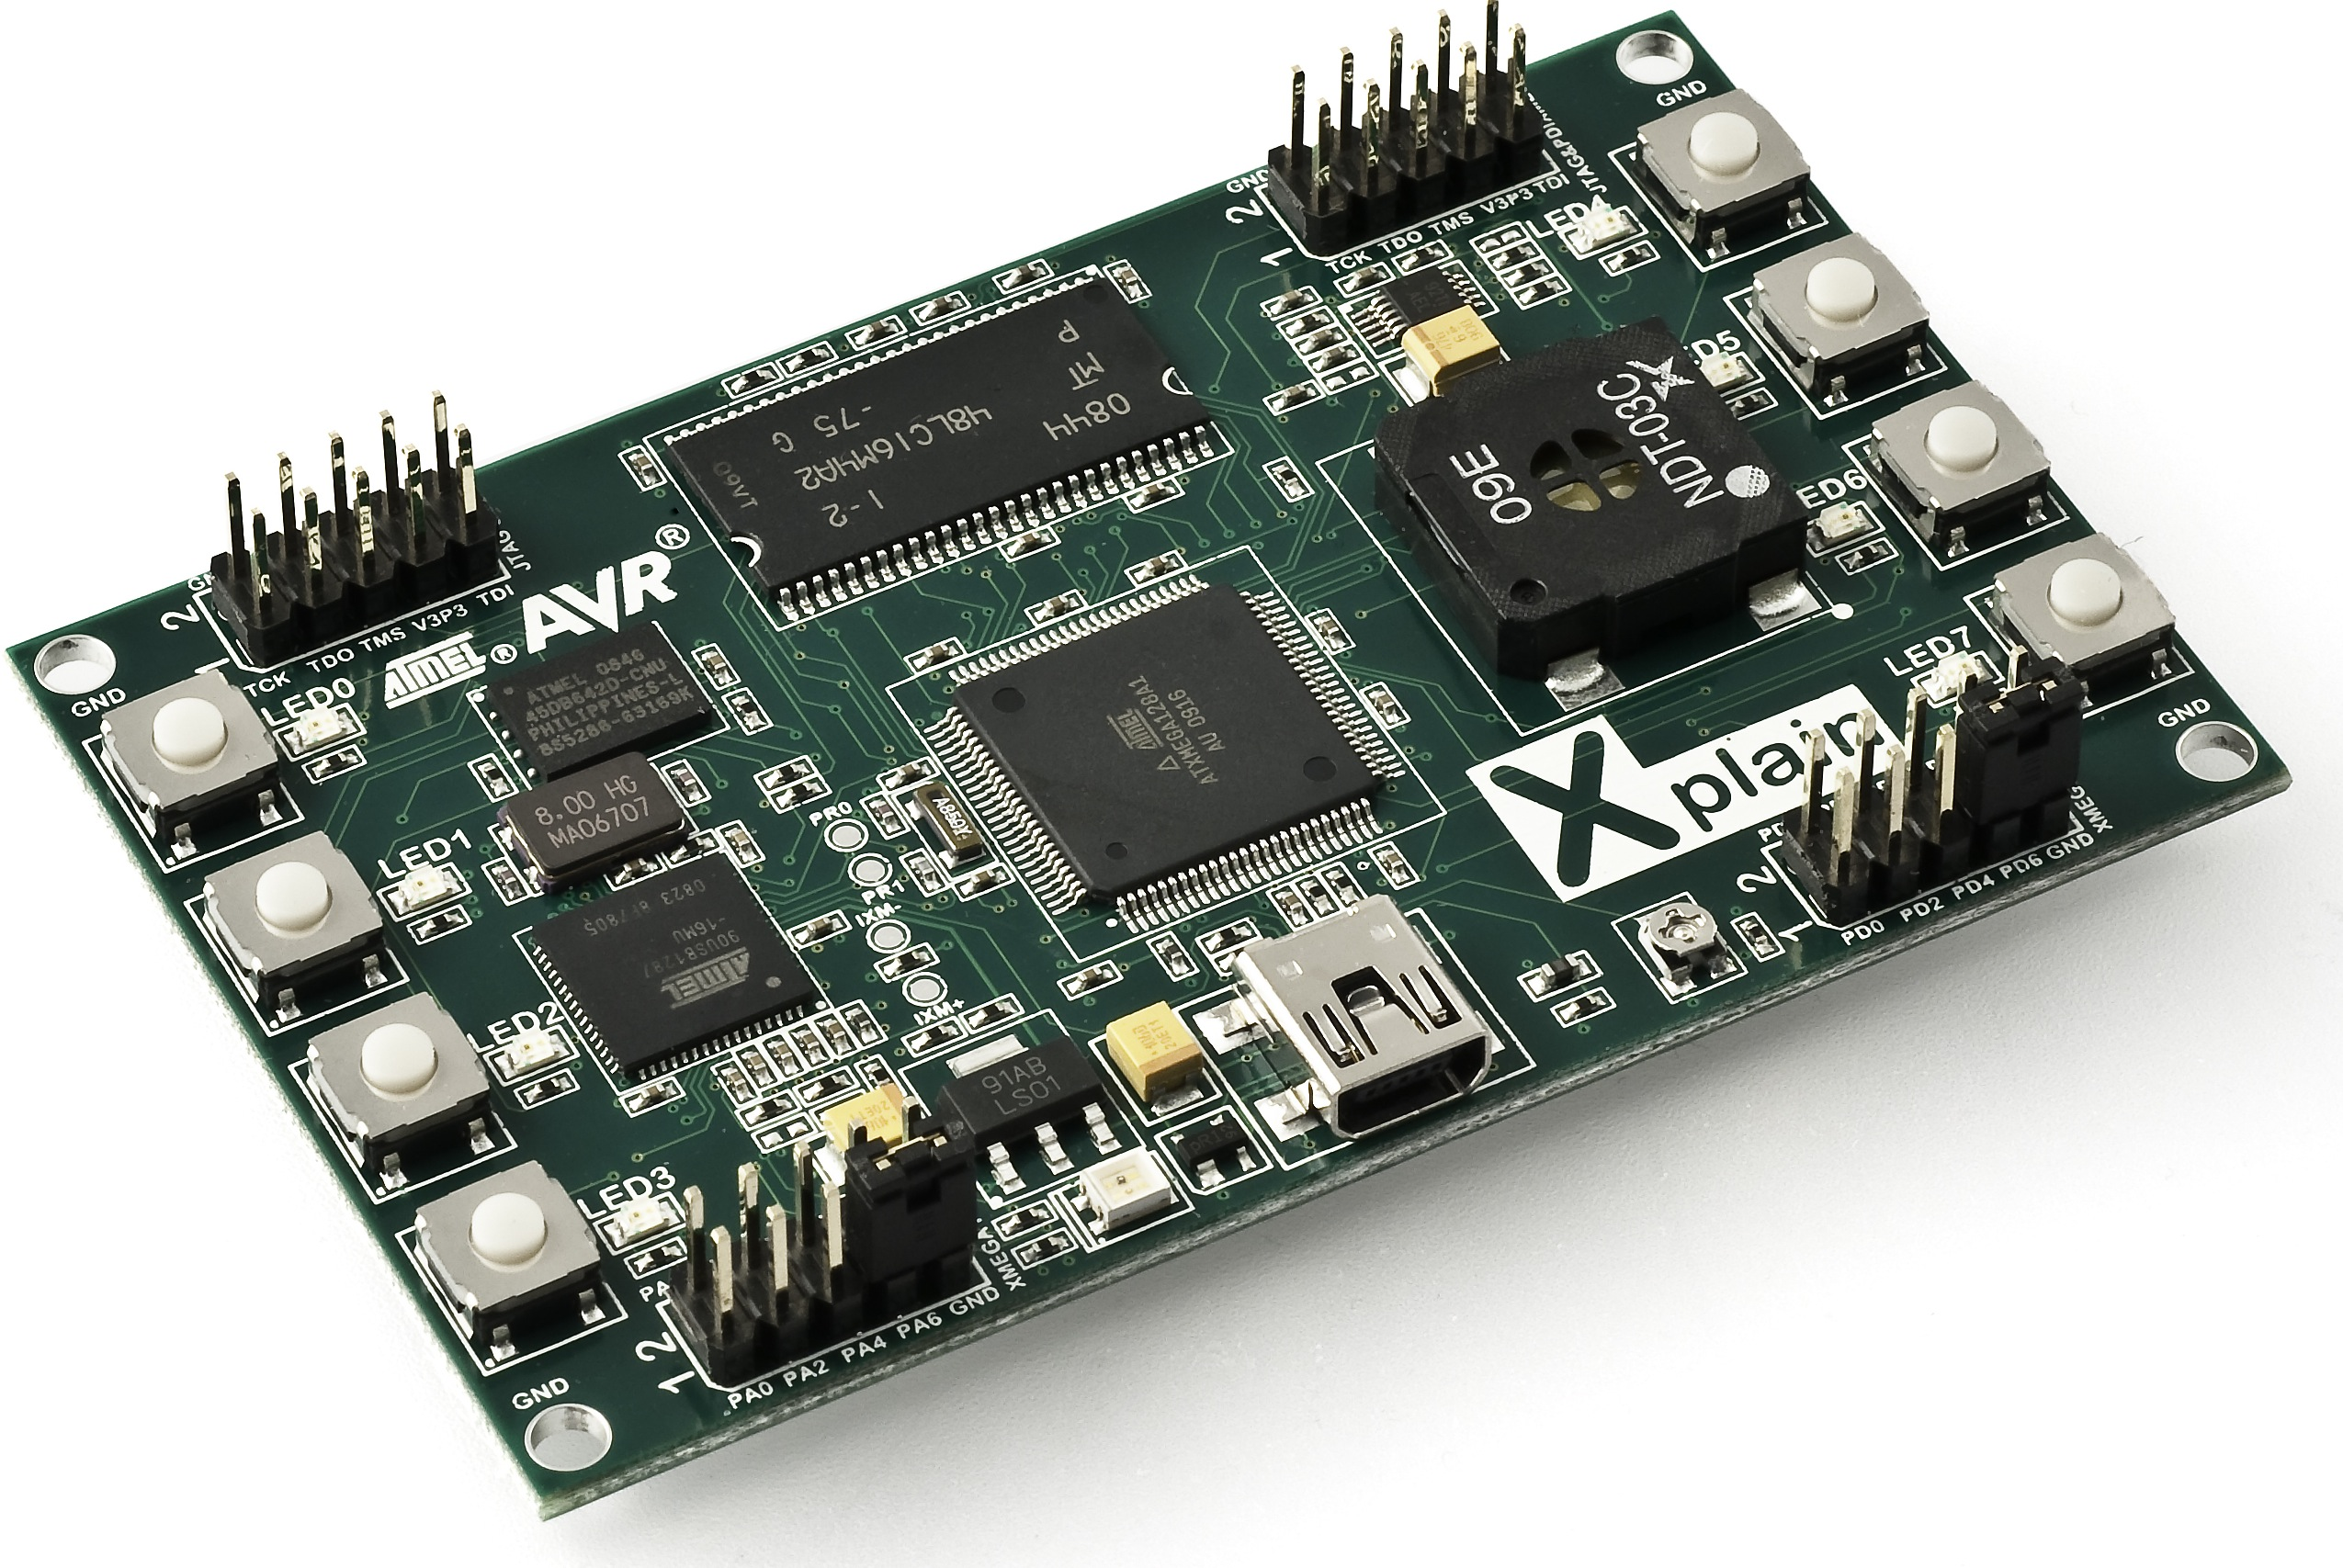
\includegraphics[width=0.4\textwidth]{images/xplain.jpg}
  \end{center}
  \caption{XPlain Development Board}
  \label{fig:xplain}
\end{wrapfigure}

When running at 32MHz with most peripherals disabled, the XMega was measured to draw 20mA of current at 3.3V. Running at 2MHz, the current draw was measured at 2mA. The XMega also has a number of power-save modes, where an ultra-low-power 32KHz oscillator is used. The data-sheet states these modes draw between 0.1 and $3\mu A$ depending on what functions are enabled, but this has not been tested. From this information, we can see that the XMega's power requirements are extremely minimal, especially when running at low clock speeds.

To see if the XMega128A1 would satisfy the cold-climate operation requirement, the Sparkfun breakout board was subjected to low temperature testing. Using frozen CO$_2$ (dry-ice), the temperature of the XMega was lowered to $-54^\circ$C. The internal 32MHz oscillator drifted upwards to 33MHz, with the XMega still continuing to function. Further details of the test process appear in  Appendix \ref{xmegadryice}.


\subsection{Signal Generator}
\begin{wrapfigure}{r}{0.3\textwidth}
  \begin{center}
    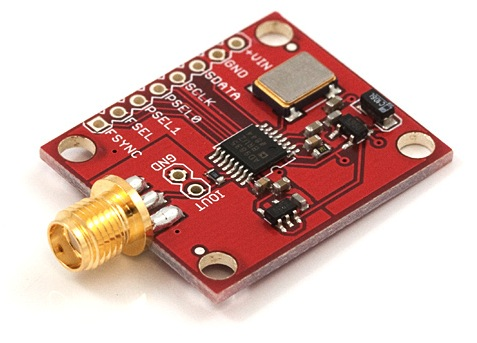
\includegraphics[width=0.28\textwidth]{images/ad9835.jpg}
  \end{center}
  \caption{AD9835 Breakout Board}
  \label{fig:ad9835}
\end{wrapfigure}
The start of the transmitter's RF section begins with the signal generator. Two signal generators were experimented with for this project, the Analog Devices AD9834 and AD9835. Both devices are programmable Direct Digital Synthesis (DDS) signal generators, able to produce sine wave output between 1Hz and 25MHz at about 0.5Vp-p.

Inside each device is a 10-bit 50Msps DAC, clocked using an external 50MHz oscillator. Serial Peripheral Interface (SPI) programmed control registers allow the programming of two different frequencies. These can be selected between using either control bits or a dedicated input pin, allowing FSK modulation. The registers can be reprogrammed approximately 7500 times per second, allowing MFSK modulation with high symbol rates. Phase registers (2 in the AD9834, 4 in the AD9835) permit BPSK and QPSK modulation, though this was not used in the project.

The AD9834 is a lower power device, drawing 8mA at 5V, while the AD9835 can draw up to 40mA. In practice, it was found that when the current draw of the required master oscillator was included, the power requirements of both devices (with supporting circuitry) were very similar (~35mA @ 5V).

The AD9835 was purchased on a breakout board from Sparkfun prior to the project, which started the idea of using a DDS to power the RF section. The AD9834 was purchased as a bare IC, and a breakout PCB was designed and constructed for it. Schematics and PCB designs for this board appear in Appendix \ref{ad9834_breakout}. The breakout was originally designed to run at 3.3v, the same voltage level as the micro-controller. However, because the board ended up using a 5V master oscillator (3.3v models were not available at the time), it had to be operated entirely at 5V. Even running at 5V the AD9834 accepts 3.3v logic levels from the XMega, unlike the 5V AD9835 which requires logic level conversion.

Being a DAC-based signal generator, the output waveform is not a pure sine. Sampling theory tells us that at 10MHz we would only 5 samples per cycle, and at 25MHz only 2 samples per cycle. At the target frequency of 7MHz, clock feedthrough (50MHz) was measured at -20dB below the target output. In Australia, spurious emissions should be -30dB below the fundamental frequency, so a reasonably sharp low-pass filter was designed to drop the clock feedthrough down by about -50dB. Use of a tuned antenna will may also attenuate the clock feedthrough enough to meet legal limits, but this could not be tested easily.

Another concern with any signal generator is how the output frequency drifts with temperature. To test this, the AD9835 was programmed to output a 7MHz sine, and was then placed in dry-ice. Over the course of an hour, the temperature of the AD9835 dropped to $-40^\circ$C, with the output frequency drifting upwards by 300Hz. This amount of drift is easily compensated for on the receiving end, and is of no concern to this project.

\begin{figure}[h]
  \begin{center}
    \includegraphics[width=0.8\textwidth]{images/ad9835_drift.pdf}
  \end{center}
  \caption{AD9835 Frequency Drift}
  \label{fig:ad9835_drift}
\end{figure}

Figure \ref{fig:ad9835_drift} shows a spectrogram of the output from a Yaesu FRG-8800 receiver as the AD9835 was cooled. Note that the frequency scale shows the demodulated frequency, with the receiver not being accurately tuned. 

\subsection{Low Pass Filter}
A low pass filter was built using a design with a cutoff frequency of about 11MHz. 

\begin{figure}[h]
  \begin{center}
    \includegraphics[width=0.4\textwidth]{images/AD9835_LPF_Schem.pdf}
  \end{center}
  \caption{AD9835 LPF Schematic}
  \label{fig:ad9835_lpf_schem}
\end{figure}

\begin{figure}[h]
  \begin{center}
    \includegraphics[width=0.7\textwidth]{images/AD9835_LPF.pdf}
  \end{center}
  \caption{AD9835 LPF Frequency Response}
  \label{fig:ad9835_lpf}
\end{figure}

The filter is composed of a 5th order low-pass filter combined with two notch filters. The rolloff is very sharp, dropping to -150dB within 8MHz, before rising again to -50dB at 40MHz. This filter has -15dB of insertion loss at 7MHz, but this can be compensated for using the following pre-amplifier.

\subsection{Pre-Amplifier}

As the output from the AD9835 (and the filter) has too little power to drive a high powered amplifier, a pre-amp needed to be built. To enable flat gain over the signal generator's wide bandwidth, an op-amp based amplifier was designed and constructed. The amplifier is based around a wide-bandwidth Analog Devices AD8008 dual op-amp IC, running from a 12V supply. Schematics of the amplifier, and a PCB design, appear in Appendix \ref{ad8008_preamp}.

The amplifier uses both op-amps in series, in a non-inverting configuration. The second op-amp is set to have a gain of 4.1, while the first has a gain variable between 3 and 20.5, giving a total gain between 12.3 and 84. The input signal is biased to half the supply voltage, to attempt to stop the signal hitting the supply or ground rails. Input and output impedances of the amplifier are both approximately $50\Omega$, 

Experimentation has found that the amplifier can be tuned to give a 4Vp-p output into a 50$\Omega$ load before distortion becomes a problem. Distortion can also occur if the supply voltage drops below 12V, as the bottom of the output waveform hits the ground rail unless the gain is lowered. Into a $50\Omega$ load this gives 40mW of RF power (16dBm), which is enough for use in some shorter range applications, but not really enough for sky-wave propagation.

\begin{figure}[h]
  \begin{center}
    \includegraphics[width=0.8\textwidth]{images/opamp_amp.jpg}
  \end{center}
  \caption{Constructed AD8008 Pre-Amplifier}
  \label{fig:ad8008}
\end{figure}

The amplifier was initially constructed on a vero-board, using a SOIC-8 (the footprint of the AD8008) to DIP breakout board. A PCB was later designed, with the breakout board still in use. This PCB was later mounted in a small jiffy box with the low pass filter. An image of the amplifier appears in Figure \ref{fig:ad8008}.

Using the AD9835 as a signal source, the gain of the amplifier was measured as being quite flat over the range of the AD9835.

INSERT AMP MEASUREMENTS HERE.

Unfortunately, the efficiency of this amplifier is quite low, running at only 8\% efficiency (40mA @ 12V). Due to the input biasing, the amplifier draws 35mA with no RF input. Short of constructing a new amplifier (which is still an option), power consumption of the amplifier can be reduced by simply cutting power to it. This is accomplished using a MOSFET switch, controlled by the CPU. 

\subsection{Class E Power Amplifier}
To provide enough power to effectively use skywave, we need more than 40mW output power. Depending on conditions, 40mW could be useful, but a few watts of output power would be preferred. To obtain this output power at maximum efficiency, a Class E MOSFET amplifier can be used.

Class E amplifier are a type of switch-mode amplifier, where the MOSFET is switched between off and saturation with a 50\% duty cycle. Unlike Class D amplifiers, Class E makes use of the output capacitance of the FET as a tuned circuit, instead of treating it as a loss. This can result in efficiencies greater than 80\%.

Two FETs were experimented with - the 2N7000 (TO-92), and the IRF510 (TO-220). The IRF510 is a common FET used in many amateur radio designs and has a high drain current rating of 5.6A. It's downside is that it has a high input capacitance - about 150pF at 7MHz. This means we need about half a watt of gate drive power to switch the FET into saturation quickly. Still, the high current rating allows for high output power from a single device - up to 10 watts is possible.

The 2N7000 is a smaller device, with only a 500mA continuous drain current rating. It's input capacitance is only about 30pF at 7MHz, meaning much less gate drive power is required. 


\subsubsection{Gate Drive}
To drive the gates of the FETs, we need a 50\% duty-cycle square wave, with sufficient power to push the FET into saturation quickly. A few methods of obtaining a square wave from the AD9835's sine output were considered, but the simplest and cheapest was to use chained schmitt triggers.

A schmitt trigger sets it's output high when the input signal rises past a certain threshold, and only sets the output low again when the input signal drops below another threshold. When fed with a correctly biased and amplified sine wave, this produces a square wave output, with exactly 50\% duty-cycle. The constructed prototype uses a 74HC14 hex-inverter, with schmitt triggering inputs. The sine-wave is biased to half the supply voltage (Logic 5V), and fed into a single inverter. The output from this inverter is then fed into the other 5 inverters, in parallel. This allows for a greater output current. The output is then capacitively coupled, and biased with an adjustable voltage divider. With the biasing set correctly, a square wave output between 3V and 8V can be produced - perfect for pushing an IRF510 into saturation. The output can also be shifted down to -1V to 4V, perfect for the 2N7000.

\begin{figure}[h]
  \begin{center}
    \includegraphics[width=0.9\textwidth]{images/FET_Driver.png}
  \end{center}
  \caption{Gate Drive Circuit}
  \label{fig:fet_drive}
\end{figure}

During construction, it was found that the output power of the inverters was still not enough to drive the FET into saturation quickly, so a push-pull buffer was constructed. This can be seen in Figure \ref{fig:fet_drive}, along with the rest of the gate driving circuitry. An LED was added between the bottom of the push-pull and ground, to add extra biasing, and to give an indication that the amplifier is running.

\subsection{Output Matching Network}

\begin{figure}[h]
  \begin{center}
    \includegraphics[width=0.8\textwidth]{images/FET_Amp.png}
  \end{center}
  \caption{Class E Amplifier}
  \label{fig:fet_amp}
\end{figure}

In Figure \ref{fig:fet_amp} we can see the circuit diagram for a Class E amplifier. L1 has a value around $50\mu$H, though this value isn't all that critical, as it just acts as a current source. Cv is tuned to make a resonant circuit with L1 and the FET's Cout at the operating frequency. The output low pass filter serves to attenuate the harmonics generated by the amplifier, leaving only the fundamental. 

\begin{figure}[h]
  \begin{center}
    \includegraphics[width=0.9\textwidth]{images/Power_Amp.pdf}
  \end{center}
  \caption{Constructed Amplifier}
  \label{fig:power_amp}
\end{figure}

A prototype amplifier was constructed using an IRF510, and this can be seen in Figure \ref{fig:power_amp}. Since toroids were not available at the time, RF choke inductors were used for L1. The output low pass filter was a copy of the filter used for the AD9835. Testing of this amplifier resulted in 880mW of output power into a $50\Omega$ dummy load, at 35\% efficiency. further investigation showed that the gate drive was still not powerful enough to drive the FET's gate, resulting in Class C operation. The RF choke inductors became noticeably warm, showing they were causing a large amount of loss in the circuit. 

\begin{figure}[h]
\begin{center}
\begin{tabular}{cc}
\includegraphics[width=7cm]{images/before_filter.jpg}&
\includegraphics[width=7cm]{images/after_filter.jpg}\\
Drain Waveform & Output Waveform\\
\end{tabular}
\end{center}
\caption{Amplifier Waveforms}
\label{fig:amp_waveforms}
\end{figure}

Figure \ref{fig:amp_waveforms} shows the drain and output waveforms of the amplifier. If the amplifier was operating as Class E, we would expect the drain waveform to be square. 

To increase the efficiency of this circuit, and to produce a proper Class E amplifier, the amplifier will be re-constructed using two 2N7000 FETs in parallel. The output filter will also be re-designed, to give a lower insertion loss. A number of toroidial cores have been ordered to make low-loss inductors, but at the time this report was written, they had not yet been received. 



\section{Software}
The hardware for this project is designed to be usable in a variety of applications, and the software is too. Hardware abstraction libraries allow easy access to I/O features of the XMega, and easy control of the signal generator. Application specific code can be built on top of these libraries, and an example application was built to demonstrate this. 

\subsection{Hardware Abstraction Libraries}
Much of the XMega's I/O is controlled by setting bits in registers. Since this is rather tedious, a number of helper libraries were written to abstract this into functions. Examples of some abstracted functions include:
\begin{packed_itemize}
\item Reading from the ADCs.
\item Writing to the DAC.
\item Writing to a UART.
\item Changing the system clock speed.
\end{packed_itemize}

\subsubsection{AD9835/AD9834 Drivers}
Since programming the signal generator ICs is a complex process, libraries were written to abstract functionality away into to a few simple functions. These include:
\begin{packed_itemize}
\item Setting a frequency or phase register.
\item Switch between frequency or phase registers.
\item Place chip in and out of sleep mode.
\item Switch between using pins or control registers.
\end{packed_itemize}

%These provide all the functionality required to perform frequency and phase modulation.

\subsection{Data Modulation}
To be able to transmit data, we need to be able to modulate the output of the signal generator in some way. Since have direct control over the signal generator's output frequency and phase, we can perform a number of types of modulation. While phase modulation (BPSK, QPSK) is possible, this project has focused on frequency shift keying.

All data modes have a setup function, and a blocking function to transmit a string (or arbitrary binary data). The setup function takes a carrier frequency as a parameter - this is the base frequency at which modulation occurs. Other parameters of the function set options such as baud rate and bandwidth.

To test reception of the data modes, existing amateur radio software (FLDigi) was used. This software can decode a large range of data modes, and can potentially be modified to support very high data-rate modes. Correct operation could be tested by either outputting RF, and using a shortwave receiver, or by setting the carrier frequency to 1KHz, and feeding the output from the signal generator directly into a computer.

\subsubsection*{Morse Code}
The first modulation mode implemented was morse code, a form of amplitude shift keying. A lookup table was used to determine the sequence of `dits' and `dahs' required, and the signal generator was switched between the carrier frequency and 0Hz (DAC-midscale) as required.

The speed (words-per-minute) of the morse code can be varied from QRSS speeds (extremely slow - $<$1 WPM) up to fast speeds (20-30 WPM). The amplitude of the signal generator can only be either full-scale or off, so the sharp amplitude changes can cause `key clicks', which cause wide-bandwidth noise to be introduced in the output signal. To fix this problem, we can key the output amplifiers on and off, instead of the signal generator. A large capacitor on the power rails will limit the amplitude rise, and limit the amount of clicking present.

Depending on key clicking and the speed used, the bandwidth required by morse code can be very small, usually only a few Hz.

\subsubsection*{RTTY - Radio TeleTYpe}
\begin{figure}[h]
  \begin{center}
    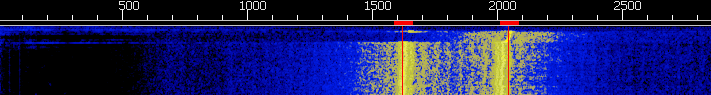
\includegraphics[width=0.9\textwidth]{images/rtty.png}
  \end{center}
  \caption{Spectrogram of a RTTY Transmission (300 baud, 425Hz shift)}
  \label{fig:rtty}
\end{figure}
RTTY, or radio-teletype, is a simple form of frequency shift keying (FSK). Two frequencies are used, representing either a logical `1' or a `0'. Stop and start bits are used to signify the start and end of a transmitter byte. By default no error correction is used, but could be added by the user.

Baud rates for this mode range from 45 up to 300 baud, with higher rates possible. The shift between the two frequencies can be set arbitrarily, but a shift equal to the baud rate or higher (in Hz) is recommended.

RTTY's bandwidth usage can vary depending on the frequency shift and baud rate in use. For example, a 300 baud transmission with a 425Hz shift uses approximately 1KHz of bandwidth. 

RTTY is not very noise resistant - a high SNR is required for correct decoding. It is recommended that some form of checksum be used in the transmission to check received data.

\subsubsection*{DominoEX}
\begin{figure}[h]
  \begin{center}
    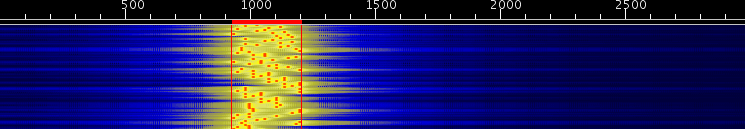
\includegraphics[width=0.9\textwidth]{images/dominoex.png}
  \end{center}
  \caption{Spectrogram of a DominoEX Transmission (7.8125 baud, 346Hz bandwidth)}
  \label{fig:dominoex}
\end{figure}
DominoEX is a MFSK (Multiple Frequency Shift Keying) data mode, developed by Murray Greenman\citep{ref:dominoex}. It uses 18 tones with incremental frequency shift keying, where the data is communicated by the difference between tones, not the tone itself.

A number of variations on DominoEX are available, with baud rates ranging from 4Hz up to 29Hz. User data throughput ranges from 3 to 16 characters per second, and bandwidth requirements range from 173 to 524Hz, depending on the mode used. 

DominoEX is more noise resistant than RTTY, but has very strict timing requirements. Small differences in tone timing (such as if an interrupt is called between tone changes) can cause the demodulator (FLDigi) to become confused and stop decoding. This issue was solved by disabling interrupts during transmission. Another solution would be to make the transmission code interrupt based, but this was not implemented.

%\subsection{Data Inputs}


\section{First Prototype \& Application Test}
To enable proper testing of the transmitter system, a prototype was constructed. The XPlain development board and the AD9835 signal generator were connected together using vero-board, with on-board 3.3V and 5V regulators to allow running everything from a 12V supply. Initially, the regulators were standard linear regulators, but switch-mode regulators were eventually purchased. These switch-mode regulators operate at approximately 80\% efficiency.

\begin{figure}[h]
  \begin{center}
    \includegraphics[width=0.9\textwidth]{images/MainBoard.pdf}
  \end{center}
  \caption{Prototype Mainboard}
  \label{fig:mainboard}
\end{figure}

Figure \ref{fig:mainboard} shows the prototype main-board. This board was connected to the amplifiers via short lengths of coaxial cable, as can be seen in Figure \ref{fig:prototype}. This figure also shows a 1:1 balun, used for matching the $50\Omega$ output to a half-wave dipole antenna (not connected in this image).

\begin{figure}[h]
  \begin{center}
    \includegraphics[width=0.9\textwidth]{images/prototype.pdf}
  \end{center}
  \caption{Assembled Prototype System}
  \label{fig:prototype}
\end{figure}


\subsection{Test Application - HAB Payload}
Mid-2010, the author became involved with a local high altitude ballooning group - Project Horus. The Project Horus group use telemetry on the 433MHz ISM band to transmit positioning and temperature data from their payloads, and were interested in other telemetry systems. Terry Baume, the founder of Project Horus, offered to fly a HF telemetry transmitter as a payload on a future launch. This would allow testing of the prototype in the harsh environments present at high altitudes. 

To be able to fly the prototype as a payload, a few additions had to be made. First was a way of getting the payloads position - a GPS module. The author already had a GPS module from another project, so this was wired into the main-board. To be able to collect information on the temperatures the payload would experience, temperature sensors (Maxim DS18B20) were added. The supply voltage was also fed into one of the ADC inputs via a voltage divider, so it can be measured. To save time, libraries to parse GPS input, and read from the temperature sensors were ported from the Arduino Project (see Appendix \ref{arduino}).

Data is collected from the inputs every few seconds, and compiled into a single line, containing information as follows:
\$\$CALLSIGN,Transmit Count, UTC Time, Latitude, Longitude, Altitude, Speed, Number of GPS Satellites in use, Internal Temperature, External Temperature, Supply Voltage * CRC16 Checksum\\
This data is then transmitted at 7.037MHz using 300 baud RTTY, with a 425Hz carrier shift.
Below is an example of a generated data sentence:
\begin{verbatim}
$$DARKSIDE,4573,07:04:04,-35.35509,138.44395,32117,98,15,6,-3,10.7*A0F0
\end{verbatim}

This format was chosen as it is mostly compliant with the UK High Altitude Society telemetry protocol\citep{ref:ukhas}. This allows the use of the `dl-fldigi' client to decode, parse, and upload the data to an online system that allows live tracking of high altitude balloons.

\begin{figure}[h]
  \begin{center}
  \begin{tabular}{cc}
    \includegraphics[width=0.685\textwidth]{images/payload_inside.jpg} &
    \includegraphics[width=0.315\textwidth]{images/payload_balloon.jpg}\\
  \end{tabular}
  \end{center}
  \caption{Prototype mounted inside payload box, and view of payload below balloon}
  \label{fig:payload_inside}
\end{figure}

The main-board and pre-amp were mounted inside a polystyrene box, along with a Lithium battery pack. The power amplifier was not included as it was not finished yet, and 40mW was deemed sufficient output power.  A small 1:1 balun was mounted to the side of the pre-amplifier, connected to a half-wave dipole extending outside of the box. An image of the constructed payload, and an image of the payload suspended below a balloon, appear in Figure \ref{fig:payload_inside}.

On the 9th of October 2010 the payload was launched as Horus 8, together with another payload containing the standard UHF telemetry system and a HD video camera. A full write-up appears in Appendix \ref{horus8}. 

The balloon and payloads rose to 32km altitude, and were successfully received all around the state. The HF payload's data was received and decoded as far away as Whyalla, in South Australia's central north, at a distance of approximately 270km. 

The balloons burst, and after a short chase the payloads ended up landing about 200m offshore, at Carrickalinga (-35.4148, 138.3231), a small beach-side down near Myponga. The payloads were successfully recovered, with only a small amount of salt-water corrosion. The HF payload survived the corrosion, and after some cleaning, works perfectly.

Throughout the test, the external temperature dropped to $-30^\circ$C. Unfortunately, due to the use of a linear regulator on the main-board (switch-mode supplies had not arrived in time), the inside of the payload only dropped to $-5^\circ$C.

\section{Testing}

\section{Project Management}

\section{References}
\renewcommand*{\refname}{\vspace*{-12mm}}
\begin{thebibliography}{99}
\bibitem{ref:iridium}
Iridium Communications Inc. ``Iridium Satellite Call Plans"" \url{http://www.iridiumphones.com.au/Call\%20Plan\%20Brochure\%20-\%20Post-paid.pdf}, 2010

\bibitem{ref:bomtx}
ACMA Register of Radio-communications Licenses, Met Bureau Site near Corkscrew Rd Montacute \url{http://web.acma.gov.au/pls/radcom/assignment\_search.lookup?pACCESS\_ID=1320447&pDEVICE\_ID=1316356}

\bibitem{ref:bom}
Australian Bureau of Meteorology, ``IPS Online HF Network Frequency Selection Tool" \url{http://www.ips.gov.au/HF\_Systems/7/1/10} , 2010 %[Mar. 14, 2010]

\bibitem{ref:dominoex}
Murray Greenman, ``DominoEX - an IFK Mode for HF'' 
\url{http://www.qsl.net/zl1bpu/MFSK/DEX.htm}

\bibitem{ref:ukhas}
UKHAS ``Communications Protocol''
\url{http://ukhas.org.uk/communication:protocol}

\end{thebibliography}


\newpage
\begin{appendices}
\section{XMega Dry Ice Testing}
\label{xmegadryice}
To test the AT-XMEGA128A1 breakout board, the chip was programmed to output the internal clock signal on a I/O pin, and one of the UARTs was programmed to continually send out ``Hello World" at 9600 baud. A LED was also attached to the board, and the chip programmed to flash it at 1Hz. The breakout board assembly was wrapped in bubble wrap (for insulation) with a ribbon cable exiting the insulation to carry the data lines. The insulated board was then placed in a small foam Eski containing approximately 3KG of dry ice. Over the course of an hour, the chip cooled down to -49$^\circ$C, where it stayed for approximately 20 minutes. After shuffling the dry ice slightly, the chip cooled down a further 5$^\circ$C, to -54$^\circ$C at which point the test was aborted. Throughout the test the clock frequency and chip temperature were measured, to produce the plot in Figure \ref{32mhzrc}.


\begin{figure}[h!]
\begin{center}
\includegraphics[width=13cm]{images/32MHzRC.pdf}
\caption{AT-XMEGA128A1 RC Clock Drift}
\label{32mhzrc}
\end{center}
\end{figure}

\begin{figure}[h!]
\begin{center}
\includegraphics[width=13cm]{images/xmega_4.jpg}
\caption{AT-XMEGA128A1 Breakout Board Wrapped in Insulation}
\label{xmega_4}
\end{center}
\end{figure}

\newpage
\begin{figure}[h!]
\begin{center}
\includegraphics[width=13cm]{images/xmega_2.jpg}
\caption{AT-XMEGA128A1 Breakout Board Warming up after testing.}
\label{xmega_2}
\end{center}
\end{figure}

\begin{figure}[h!]
\begin{center}
\includegraphics[width=11cm]{images/xmega_3.jpg}
\caption{Ice forming on the XMEGA's pin headers after testing.}
\label{xmega_3}
\end{center}
\end{figure}

\newpage
\section{Software}
All software for this project has been released under the GPLv3 license. 

\subsection{The Arduino Project and the XMega}
\label{arduino}
The Arduino is an open-source electronics prototyping platform based on flexible, easy-to-use hardware and software.
Since many users of the Arduino haven't had much experience in programming, many libraries have been created to fulfil various needs. It's fairly common to begin working on a bit of code to drive some chip, to find that someone has already written a library a few months previously. To quickly get sections of the XMega's codebase working, it was decided to port certain Arduino libraries to the XMega platform. 

Arduino's IDE uses the `wiring' programming language. Wiring is a `C-like' language, following most of C's syntax, to the point that the Arduino IDE uses a collection of C++ libraries to `convert' wiring to C++ for compilation. While these libraries could be ported to the XMega allowing usage of the Arduino IDE for this project, this would have required a lot of work and been out of scope. Instead, the Arduino libraries which were needed (OneWire, DallasTemperature, TinyGPS) were individually ported. This involved replacing various Arduino-specific function calls with generic AVR-C calls, and some other minor code changes. 

\newpage
\section{Schematics \& PCBs}
\subsection{AD8008 Pre-Amp}
\label{ad8008_preamp}
\begin{figure}[h!]
\begin{center}
\includegraphics[width=12cm]{images/AD8008_Schem.pdf}
\caption{AD8008 Pre-Amp Schematic}
\label{ad8008_schem}
\end{center}
\end{figure}
\begin{figure}[h!]
\begin{center}
\includegraphics[width=12cm]{images/AD8008_PCB.pdf}
\caption{AD8008 Pre-Amp PCB Artwork}
\label{ad8008_PCB}
\end{center}
\end{figure}
\newpage
\subsection{AD9834 Breakout Board}
\label{ad9834_breakout}
\begin{figure}[h!]
\begin{center}
\includegraphics[width=12cm]{images/AD9834_Schem.pdf}
\caption{AD9834 Breakout Board Schematic}
\label{ad9834_schem}
\end{center}
\end{figure}
\begin{figure}[h!]
\begin{center}
\includegraphics[width=12cm]{images/AD9834_PCB.pdf}
\caption{AD9834 Breakout Board PCB Artwork}
\label{ad9834_PCB}
\end{center}
\end{figure}

\section{Project Horus Launch 8 Write-up}
\label{horus8}


\end{appendices}

\end{document}